\section{Whose views do current LMs express?}
\label{sec:analysis}

We now evaluate existing models on \bname and analyze their opinion agreement with respect to people in the US. 
We study a set of 9 LMs---with different providers (OpenAI and AI21 Labs), scales (350M to 178B parameters), data collection, and training strategies.
These models can be roughly grouped into (i) base LMs, that have only been pre-trained on internet data (\model{ada}, \model{davinci}, \model{davinci}, \model{j1-grande} and \model{j1-jumbo}), and (ii) human feedback (HF)-tuned LMs that have been adapted to be more human-aligned using supervised or reinforcement learning (\model{text-*} and \model{j1-grande-v2-beta})~\citep{ouyang2022training,ai21instructbeta}\footnote{these classifications are based on public information from vendors, but due to incomplete model descriptions, it is possible that some models such as \model{j1-grande} are also instruction tuned}.


\begin{figure*}[!t]
    \vskip 0.2in
    \begin{center}
    \centerline{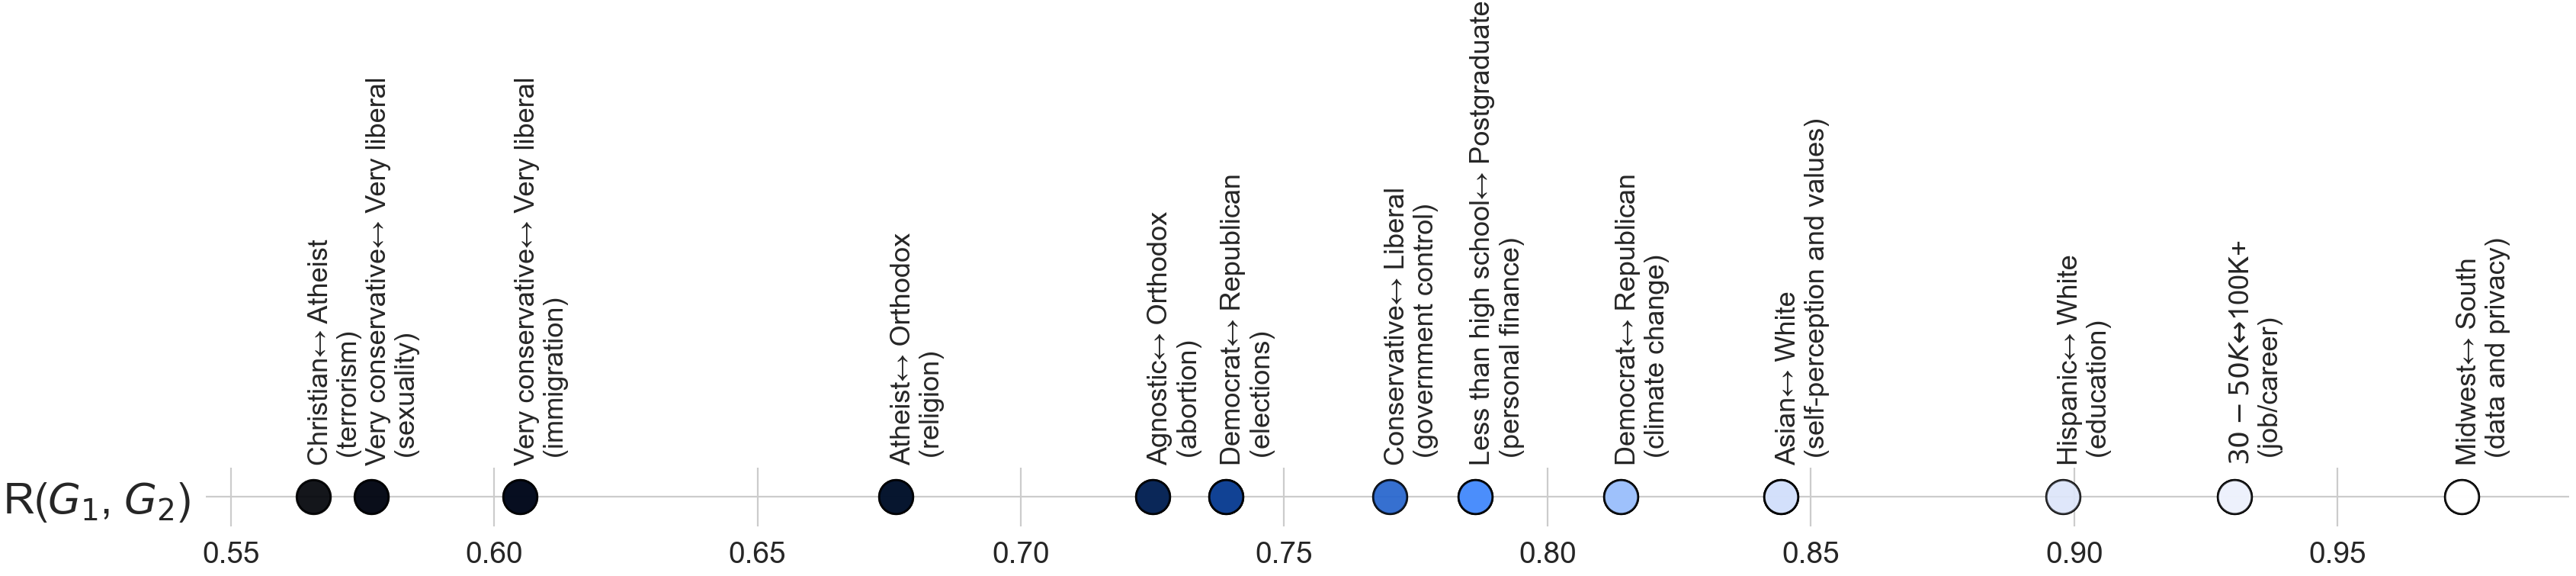
\includegraphics[width=0.9\textwidth]{Figures/calibration_bar.png}}
    \vskip 0.051in
    \centerline{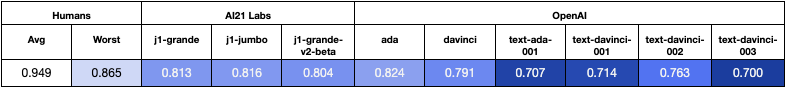
\includegraphics[width=0.95\textwidth]{Figures/representativeness.png}}
    \caption{Overall representativeness $\mathcal{R}^{\text{O}}_m$ of LMs: A higher score (lighter) indicates that, on average across the dataset, the LM's opinion distribution is more similar to that of the total population of survey respondents (Section~\ref{sec:rep}). 
    For context, we show the representativeness measures for: (i) demographic groups that are randomly chosen (`avg') and least representative of the overall US population (`worst'), and (ii) pairs of demographic groups on topics of interest. 
    }
    \label{fig:alignment_basic}
    \end{center}
    \vskip -0.2in
\end{figure*}


\paragraph{Robustness.}
\label{sec:robustness}
In general, LMs can be somewhat sensitive to the formatting of their input prompt~\citep{jiang2020can}.
We ensure that all our subsequent results are robust to such design choices by replicating our analysis with (i) different prompt templates, and (ii) permuting the order in which answer choices are presented to the model---see Appendix~\ref{app:robustness}.

\subsection{Representativeness}
\label{sec:rep}

We begin by analyzing the default representativeness of LMs,  at an overall (\emph{does its opinion distribution match that of the overall US populace?}) and group level (\emph{does it match a particular group's opinion?}).
To measure this, we evaluate model opinion distribution on \bname questions \emph{without} any context (beyond the question itself).

\paragraph{The metric.} We define the representativeness of an LM with respect to the overall population as the average alignment (Section~\ref{sec:metric})---across questions---between the default opinion distribution of the model and that of the overall population, \ie, 
\begin{equation}
    \mathcal{R}^{O}_m(Q) = \simi(D_m, D_O, Q).
  \end{equation}

Analogously, we can define the group representativeness of an LM w.r.t. to a particular demographic group $G$ as $\mathcal{R}^G_m(Q) := \simi(D_m, D_G, Q)$.
A higher overall (group) representativeness score indicates that out-of-the-box, the LM is better aligned with the distribution of viewpoints held by the overall US populace (that group).
While the maximum possible of this score is 1, it cannot be achieved for \emph{all} of the groups.
This is due to the fact that there are irreconcilable differences between the opinions of certain groups (\eg, Democrats and Republicans on guns in Figure~\ref{fig:prompt_example})---making it impossible for the model's opinion distribution $D_m$ to simultaneously match all of them.



\paragraph{Are current LMs representative?}
Figure~\ref{fig:alignment_basic} depicts the overall representativeness scores $\mathcal{R}^{O}_m$ of different LMs.
Overall, we observe that none of the models are perfectly representative of the general populace (of survey respondents).
In fact, more recent models trained to be more human-aligned~\citep{ouyang2022training,ai21instructbeta} are actually \emph{worse}---cf. OpenAI's \model{text-davinci-003} and \model{davinci} models.
To put these results into context, we compare them to salient human baselines:
\begin{itemize}
  \item First, we consider the alignment between the opinions of a each of our 60 demographic groups and the general populace ($\mathcal{R}^{O}_{G}(Q) = \simi(D_{G}, D_O, Q)$). We see that every one of these groups is \emph{more} representative of the overall populace than \emph{any} of the LMs we consider (i.e., cf. representativeness scores of `human (worst)` to all the LMs).
  \item Second, we construct a scale of alignment values between pairs of demographic groups on questions from specific contentious topics ($\mathcal{R}^{G_1}_{G_2}(Q_T) = \simi(D_{G_1}, D_{G_2}, Q_T)$). On this scale, we see that $\mathcal{R}^{O}_m$ for most models is comparable to the opinion alignment of agnostic and orthodox people on abortion or Democrats and Republicans on climate change.
\end{itemize}


\begin{figure}[!t]
    \vskip 0.2in
    \begin{center}
      \begin{subfigure}[b]{0.47\textwidth}
        \centering
        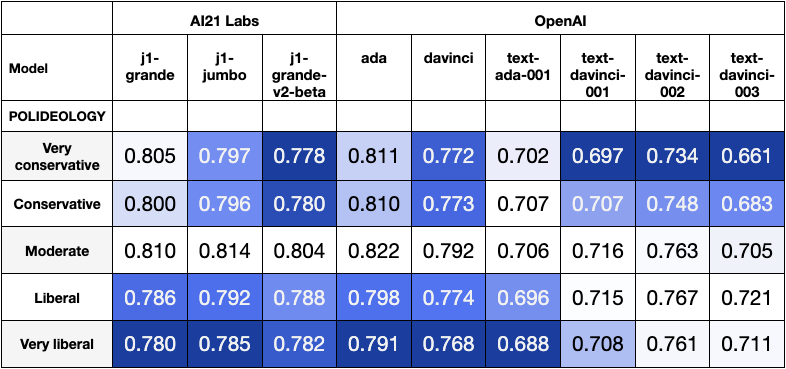
\includegraphics[width=1\columnwidth]{Figures/representativeness_POLIDEOLOGY.png}
      \end{subfigure} \hfil
      \begin{subfigure}[b]{0.485\textwidth}
        \centering
        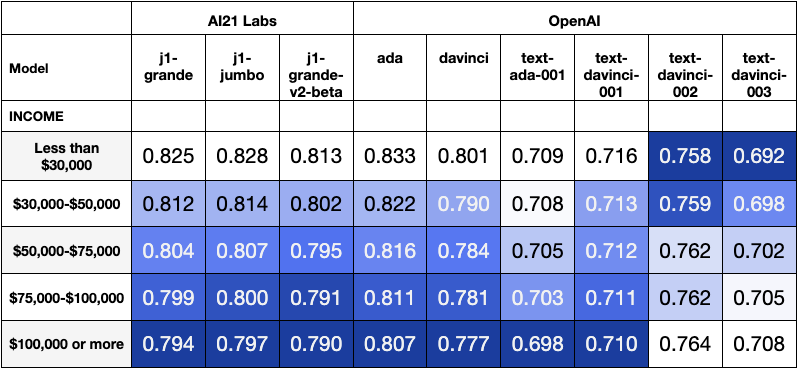
\includegraphics[width=1\columnwidth]{Figures/representativeness_INCOME.png}
      \end{subfigure}
    \caption{Group representativeness scores $\mathcal{R}^{G}_m$ of LMs as a function of political ideology and income: A higher score (lighter) indicates that, on average across dataset questions, the LMs opinion distribution is more similar to that of survey respondents from the specified group (\ie, $\mathcal{R}^G_m(Q)$ is larger). The coloring is normalized by column to highlight the groups a given model (column) is most/least aligned to. We find that the demographic groups with the highest representativeness shift from base LM (moderate to conservative with low income) to the RLHF trained ones (liberal and high income). Other demographic categories are shown in Appendix~\ref{figapp:per_md_alignment}.
      }
    \label{fig:per_md_alignment}
    \end{center}
    \vskip -0.2in
\end{figure}


\paragraph{Group representativeness.} The group representativeness scores for all the base LMs share striking similarities---\eg, being most aligned with lower income, moderate, and Protestant or Roman Catholic groups. 
This might be because all these models were trained on  snapshots of the internet---and thus mimic similar pools of human writers.
While AI21's HF-tuned model (\texttt{j1-grande-v2-beta}) behaves similarly to base LMs, the corresponding OpenAI instruct series models (\texttt{text-*}) are markedly different.
The opinions reflected by these models align more with people who are liberal, high income, well-educated, and not religious or belong to religions other than Buddhists, Muslims, and Hindus.
These groups line up with the demographics of the crowd-workers reported in OpenAI's InstructGPT paper~\citep{ouyang2022training}---\eg, predominantly young Southeast Asian and White with a college degree\footnote{While our results agree with the crowdworker demographics in the instructGPT paper, we cannot draw the conclusion that our approach recovers the RLHF crowdworker distribution, as the datasets and crowdworkers used in OpenAI's production systems are not public.}.
Finally, a broader analysis across all the groups in the Pew survey highlights several that have low representativeness scores for all LMs, such as individuals of age 65+, widowed, and high religious attendance (Appendix~\ref{figapp:per_md_alignment}). In the case of age, the InstructGPT paper similarly shows that there were almost no individuals of age 65+ that were part of the crowdsourcing process, and it is likely that the other groups (widowed, high religious attendance) may also be difficult to recruit through standard crowdsourcing vendors.


\begin{figure}[!t]
    \vskip 0.2in
    \begin{center}
      \begin{subfigure}[b]{0.45\textwidth}
        \centering
        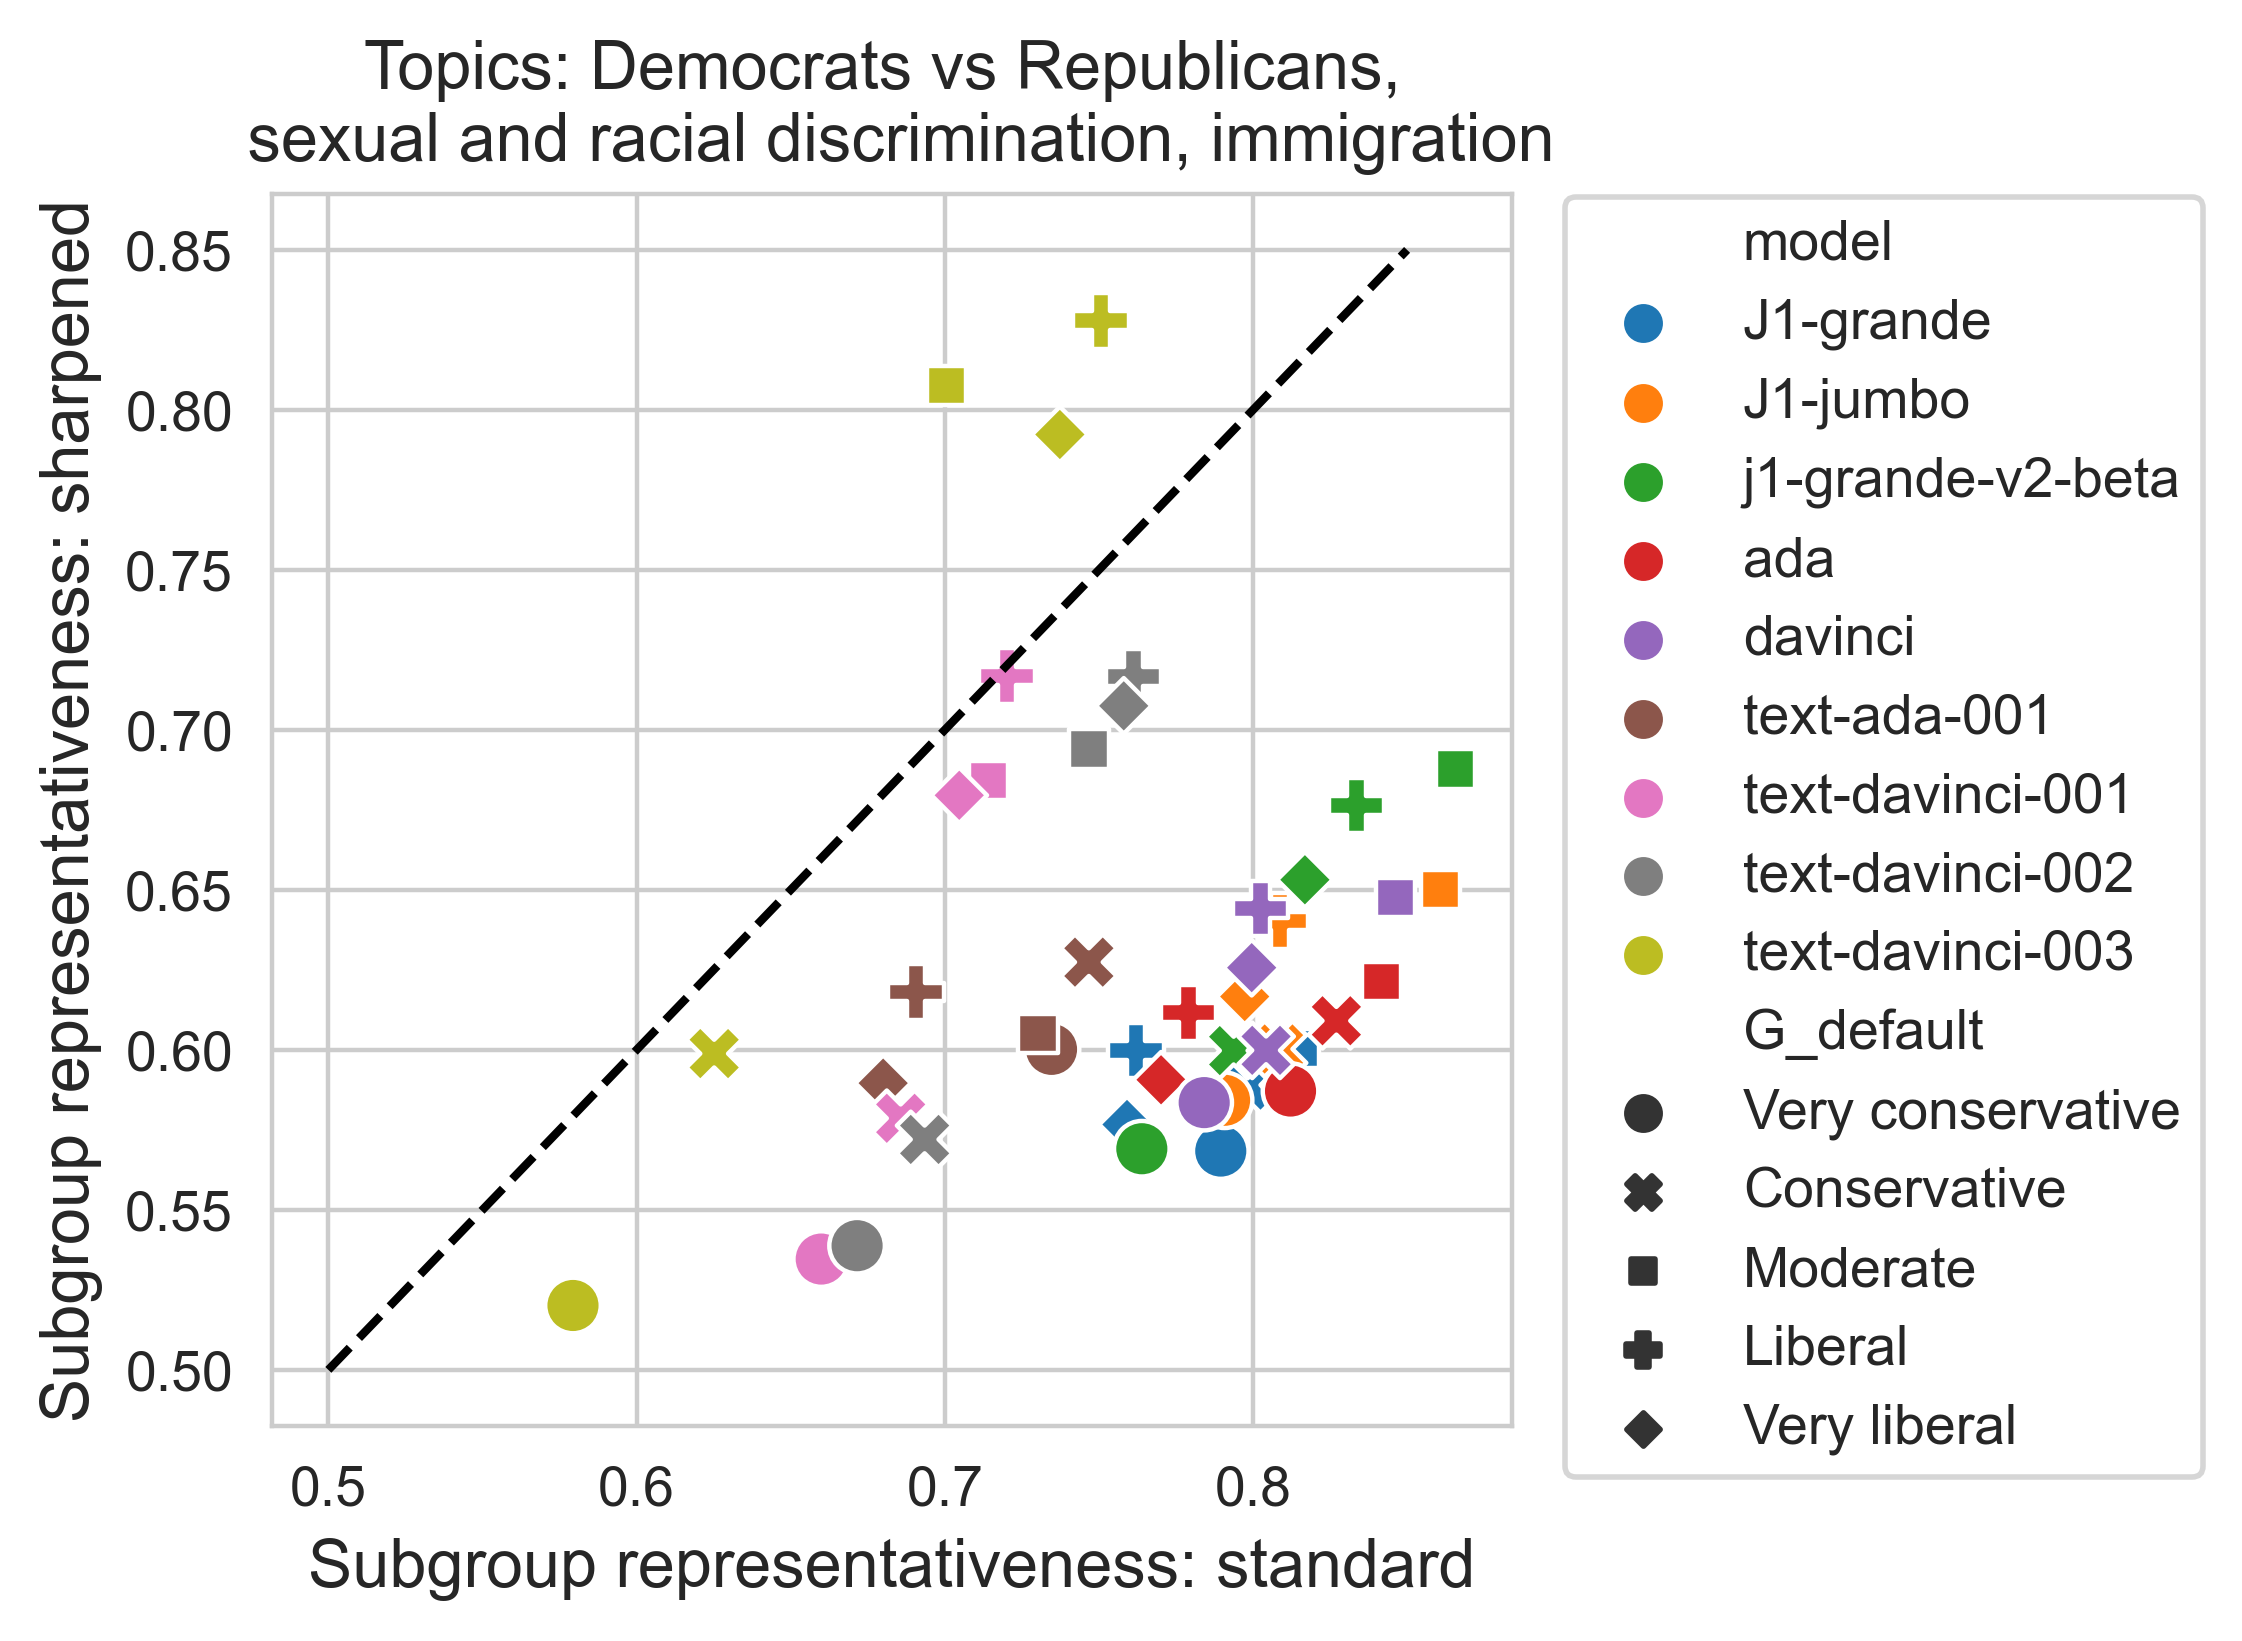
\includegraphics[width=1\columnwidth]{Figures/caricature.png}
        \caption{}
        \label{fig:polarized_alignment}
      \end{subfigure} \hfil
      \begin{subfigure}[b]{0.48\textwidth}
        \centering
        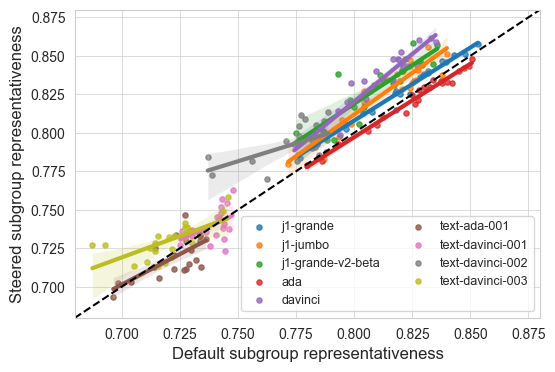
\includegraphics[width=1\columnwidth]{Figures/steerability.png}
        \caption{}
        \label{fig:steerability_overall}
      \end{subfigure} 
    \end{center}
    \caption{(a) The alignment of LM opinions with the actual and modal views of different ideological groups on contentious topics. (b) Steerability of LMs towards specific demographic groups: we compare the group representativeness of models by default (x-axis, $\mathcal{R}^G_m$) and with steering $\steer^G_m$ (y-axis). Each point represents a choice of model $m$ and target group $G$, and points above the $x=y$ line indicate pairs where the model's opinion alignment improves under steering. Shaded lines indicate linear trends for each model $m$, and we generally observe that models improve from steering (above $x=y$) but the amount of improvement is limited.}
    \vskip -0.2in
\end{figure}


\paragraph{Modal representativeness.}
\label{sec:polarization}
In Figures~\ref{fig:alignment_basic} and~\ref{fig:per_md_alignment}, we saw that human-feedback tuned models (and most notably \model{text-davinci-003}) are \emph{less representative} of overall opinions.
A closer look at \texttt{text-davinci-003}'s opinion distribution provides some insight into why this might be the case.
Specifically, it has an extremely sharp (and low entropy) opinion distribution for most questions (Appendix Figure~\ref{figapp:entropy})---it typically assigns $>0.99$ probability to one of the options.
This is unlike humans, who even on contentious topics (like gun rights), tend to exhibit some diversity in opinions (see the Democratic respondent distribution in Figure~\ref{fig:prompt_example}).
This prompts us to ask: is \texttt{text-davinci-003} actually unrepresentative, or does it collapse to the most-frequent and \emph{modal} opinion of certain groups?
To test this, we construct a ``modal'' opinion distribution of a group by applying temperature scaling to the group's opinion distribution $D_G(q)$ (Appendix~\ref{app:temp}).
In Figure~\ref{fig:polarized_alignment}, we then compare the relative tendencies of LMs to match the actual and modal opinions of different political groups on contentious topics.


We observe that the behavior of \model{text-davinci-003} is quite unique: its opinion distribution seems to converge to the modal views of liberals and moderates.
This indicates that the dominant approach of aligning LMs with RL based human-feedback not only skews the model's opinions towards certain groups (liberals), but also pushes the model to almost embody caricatures of those groups (\eg, 99\% approval of Joe Biden).
From a different standpoint, this finding highlights the importance of considering the entire spectrum of human responses rather than just the mode. A modal analysis of \texttt{text-davinci-003} would conclude that the model is highly representative of Democrats, where in reality its representation collapses the diversity of opinions held by different democrats into a single, modal response.

\paragraph{Refusals.}
In our comparison of human and LM opinions so far, we omitted the ``refusal'' option for all questions due to its non-ordinal nature.
In Appendix~\ref{app:refusal}, we thus separately compare the refusal rates of LMs and human respondents. 
We find that all models have low refusal rates. 
Although human feedback-tuned models are encouraged to refuse to take a stance on contentious issues~\citep{askell2021general,ouyang2022training}, they tend to rarely do so in our multiple-choice setting---with refusal rates as low as 1--2\%.
\subsection{Steerability}
\label{sec:steerable}
\label{sec:steering}
We now shift our focus from measuring the default alignment of LM opinions with those of various demographics groups \emph{without} prompting, to studying their steerability \emph{with} group-specific prompting. This is especially important in settings such as personalization, where
a key measure of performance is an LM's ability to adapt to represent the opinion of various demographic groups.

\paragraph{The metric.} We measure steerability as the average opinion alignment, across dataset questions, between an LM and a particular demographic group $G$ -- where the model is prompted with group information in its context.
Since our goal is to test whether a model \emph{can} be steered toward a group, we consider three prompting strategies---\textsc{QA},\textsc{BIO},\textsc{PORTRAY} (see Section~\ref{sec:prompting})---for each question and choose the one that works best.
Concretely, we measure steerability as:

\begin{equation}
    \steer^{G}_m(Q) =  \frac{1}{|Q|} \sum_{q \in Q} \max_{c_G \in \small{[\textsc{QA},\textsc{BIO},\textsc{POR}]}} \simi(D_m(q; c_G), D_{G}(q))  \nonumber
\end{equation}
where $D_m(q; c_G)$ denotes the LM opinion distribution conditioned on the group-specific context $c_G$.
A higher $\steer^{G}_m$ score indicates that the model is better aligned to the opinions of the given group.
Note that unlike default subgroup representativeness, an LM's steerability could be simultaneously high for multiple (disagreeing) groups.
In fact, in many cases, we might want disparities in the default subgroup representativeness scores of an LM to be remedied by steering.


\paragraph{Steering does not solve opinion misalignment.}

We attempt to steer current LMs towards one of 22 demographic groups (\eg, Republican, Asian, Jewish) listed in Appendix Table~\ref{tab:steer_groups} on a subset $Q_S$ of 500 highly contentious questions from \bname.
In Figure~\ref{fig:steerability_overall}, we compare different LMs in terms of their ability to match the opinions of a subgroup on these questions, by default and with steering ($\steer^{G}_m(Q_S)$ from Section~\ref{sec:rep}).

Most LMs (with the exception of \model{ada}) do become somewhat more representative of a subpopulation post-steering.
However, none of the disparities in group opinion alignment of an LM disappear after steering, with \model{text-davinci-002} showing the smallest post-steering alignment gap across groups. In most cases, we see the representativeness of all groups improving by a constant factor---indicating that the LM still does better on some groups than others.
In Appendix Figure~\ref{figapp:steerability_group}, we visualize which LMs are most effective at adapting towards a particular group: \eg, \model{j1-grande-v2-beta} for Southerners and \model{text-davinci-002} for liberals.


\subsection{Consistency}
\label{sec:consistency}

\newcommand{\consis}{\mathcal{C}}


\begin{figure*}[!t]
    \vskip 0.2in
    \begin{center}
    \centering
    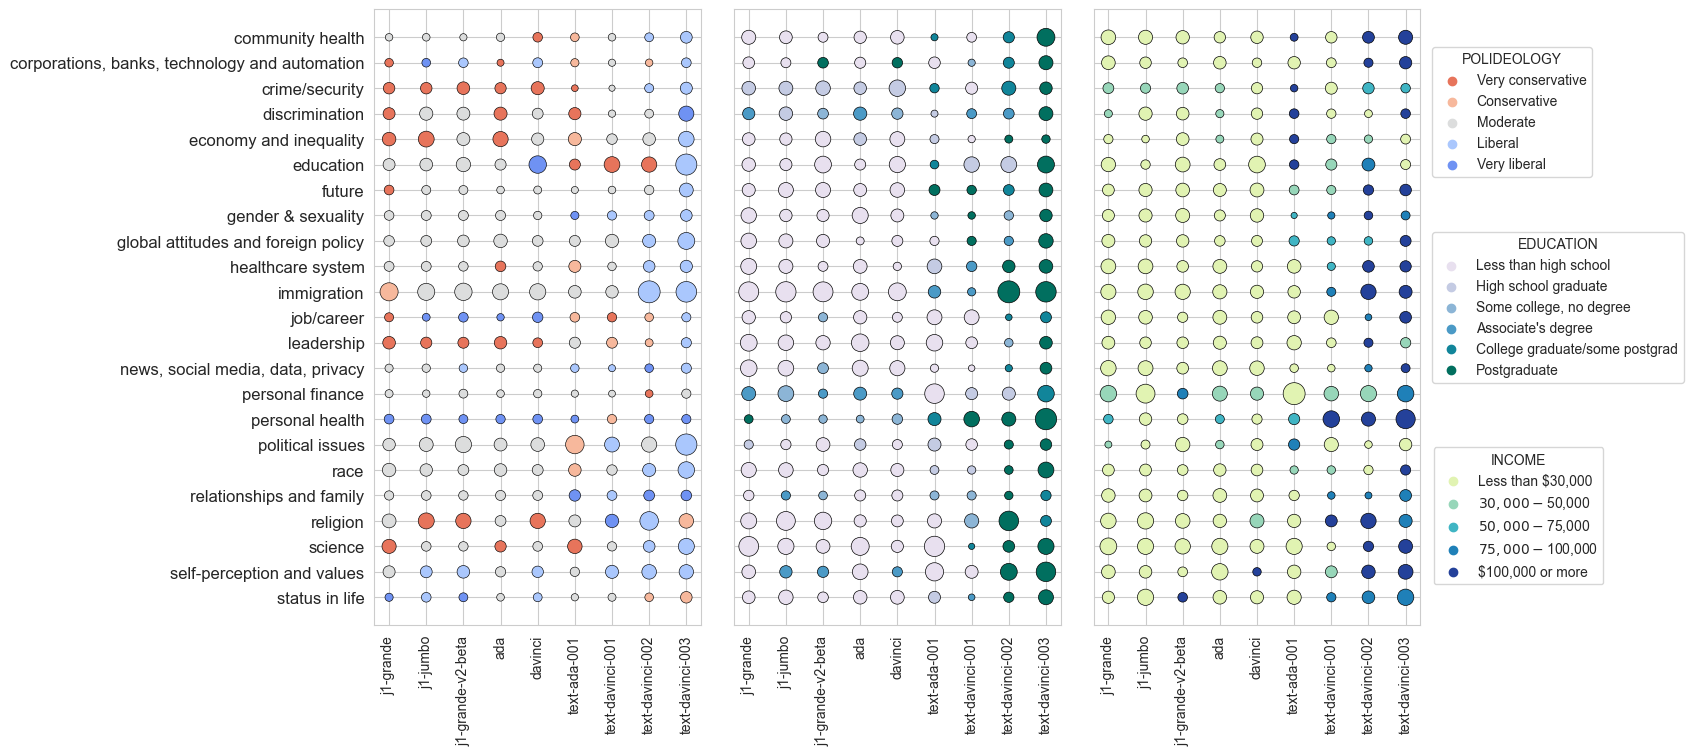
\includegraphics[width=1\textwidth]{Figures/consistency_cg.png}
    \caption{
      Consistency of different LMs (columns) across topics (rows) on different demographic attributes (panels). Each dot indicates an LM-topic pair, with the color indicating the group to which the model is best aligned, and the size of the dot indicates the strength of this alignment (computed as the ratio of the best and worst subgroup representativeness for that topic, see Appendix~\ref{app:consistency} for details). We find significant topic-level inconsistencies, especially for base LMs, and strong educational attainment consistency for RLHF trained LMs.}
    \label{fig:topic_ideology}
    \end{center}
    \vskip -0.2in
\end{figure*}



Our earlier default representativeness analysis (Section~\ref{sec:rep}) showed marked skews in the views expressed by LMs, with base LMs reflecting opinions consistent with lower income and education and the opposite for human-feedback tuned ones.
However, we might want to go beyond this aggregate analysis and ask:  \emph{are the views expressed by LMs consistent across topics?}~\citep{saris2004studies}.
For instance, is \model{text-davinci-002} politically Liberal on all matters or does it take a Conservative stance in some cases?
We now leverage the fine-grained topic taxonomy in our \bname dataset to answer this question.
To this end, we  inspect human-LM opinion similarity on a topic level by computing alignment on a subset of questions $Q_T$.



\paragraph{Are LMs consistent?}
In Figure~\ref{fig:topic_ideology}, we break down the subgroups that various LMs (columns) most closely align to (colors) across 23 topic categories (rows) by political ideology, education and income. 
Of all the LMs we study, the base models from both providers and the RLHF-trained \model{text-davinci-003} from OpenAI seem to be the most consistent -- albeit towards different sets of groups.
None of the models are perfectly consistent however, and even \model{text-davinci-00\{2,3\}} aligns with conservatives on topics like religion.

\paragraph{The metric.}
To distill these trends into a single measure, we ask what is the fraction of topics for which an LM's most aligned group overall (weighting topics equally) matches the LM's most aligned group on the given topic (with questions $Q_t$).
Specifically, for a model, we first identify the group it best aligns to across topics as 
\begin{equation*} 
  G_m^{best} := \argmax_{G} \left( \frac{1}{T} \sum_{T'}\mathcal{R}^{G}_M(Q_{T'}) \right)  
\end{equation*}
\noindent We then define consistency as:
\begin{equation*} 
\consis_m := \frac{1}{T}\sum_{T} \mathbbm{1} \left [ \left(\argmax_{G} \mathcal{R}^{G}_M(Q_T)\right)  = G_m^{best}  \right ] %
\end{equation*}
Our metric $\consis_m$ is bounded between 0 and 1, and a higher score implies that the model agrees with the views of the same subgroups across all topics.
In Figure~\ref{fig:inconsistency}, we visualize the average consistency score of a model across demographic traits (religion/income/ideology, etc). We find that the overall consistency scores of current LMs are fairly low---indicating that they are expressing a patchwork of disparate opinions.
Note that this may not always be problematic---after all even individuals can hold seemingly inconsistent beliefs.

\begin{figure*}[!t]
    \vskip 0.2in
    \begin{center}
    \centerline{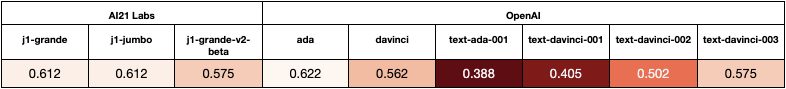
\includegraphics[width=0.95\textwidth]{Figures/consistency.png}}
      \caption{Consistency of LM opinions $\consis_m$, where a higher score (lighter) indicates that an LM aligns with the same set of groups across topics.
      }
    \label{fig:inconsistency}
    \end{center}
    \vskip -0.2in
\end{figure*}



















